%\section{Shared Environmental Forcing}
%
%First, we test the hypothesis that Fraser River sockeye salmon show shared environmental forcing. Using the framework of empirical dynamic modeling (EDM) [ref], we apply the method of ``dewdrop regression'' to test for dynamic similarity.
%
%% how dewdrop regression works and how we apply it here
%
%Thus, the similarity in dynamics can be tested by partitioning the time series data accordingly as either the library or prediction set.
%
%We first subset the data according to stock and cycle line. Since the majority of salmon in this system recruit at age-4, we can consider the annual time series of age-4 recruits as 4 time series that ``time-share'' the same spawning regions.
%
%We then consider forecasts for each stock-cycle-line unit (``subunit'') using a library composed of different subunits:
%\begin{itemize}
%\item Model 1: the library is composed of subunits from the same stock (but different cycle lines)
%\item Model 2: the library is composed of subunits from the same cycle line (but different stocks)
%\item Model 3: the library is composed of any other subunits
%\end{itemize}
%
%The performance of these three models can be compared:  if the fish in each stock exhibit different migratory behaviors or mortality is heavily dependent on conditions unique to each stock, then we would expect model 1 to perform better.  If instead, mortality is primarily dependent upon oceanic conditions which vary from year to year, then we would expect model 2 to perform better.  However, if all cycles contained similar dynamics, then we would expect the three models to have equal performance.  (Alternatively, if each cycle had different dynamics, the three models would also have equal performance, but predictability would be low.  To differentiate this situation from the the case where all cycle lines have similar dynamics, we can compare the performance of model 3 with that of a univariate model that uses a cycle line to predict itself.  If the two predictabilities are equal, then the other cycle lines have an equivalent amount of dynamic information useful for prediction, suggesting that all cycle lines are dynamically similar.)
%
%\subsection{Results}
%
%\begin{figure}[!ht]
%\begin{center}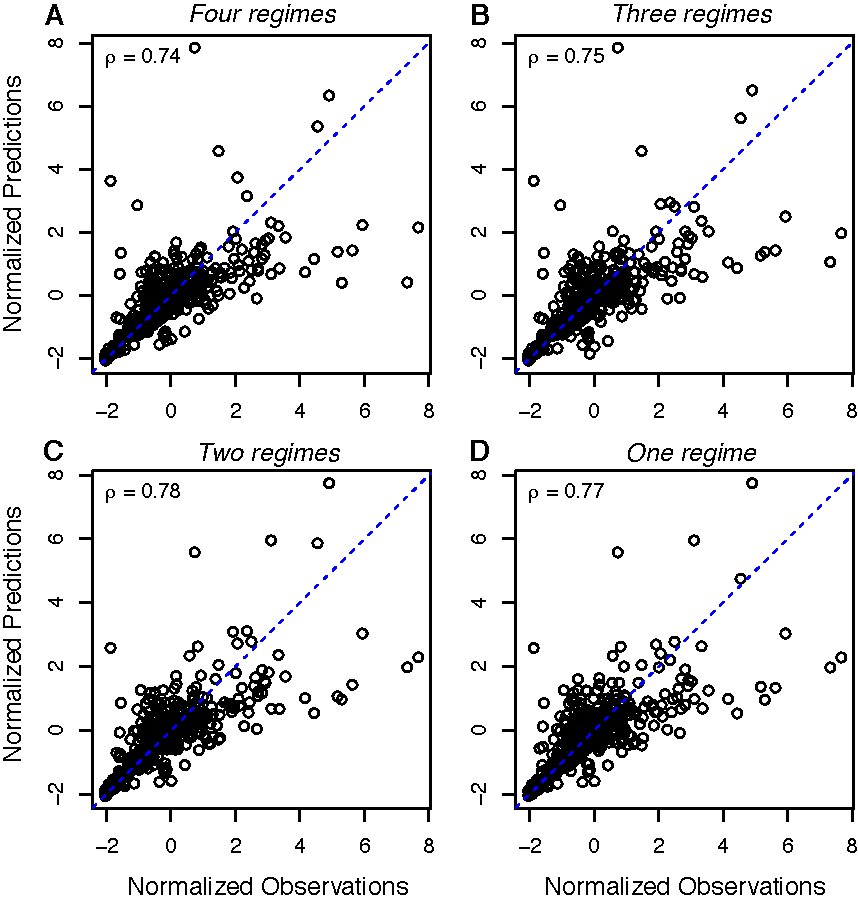
\includegraphics[width=\maxwidth{\textwidth}]{fig_regimes_1.pdf}\end{center}
%\caption{Correlation coefficients ($\rho$) for predictions made by different models.  The bottom, middle, and top of each box represent the lower-quartile, median, and upper-quartile respectively of $\rho$ for each model.}
%\label{fig_salmon_dynamic_similarity}
%\end{figure}
%
%I computed the performance (Figure \ref{fig_salmon_dynamic_similarity}) of these three models ("same stock", "same cycle year", "all cycle lines") using data consisting of 9 time series representing yearly returns of the 9 most abundant stocks (Birkenhead, Chilko, Early Stuart, Late Shuswap, Late Stuart, Quesnel, Seymour, Stellako, Weaver) from 1948-2007 (60 years).  From these time series, I extracted 36 total cycle lines corresponding to each stock and the initial year of data. (e.g. Early Stuart 1948 consists of the returns of the Early Stuart stock in 1948, 1952, 1956, ...) For the purposes of making equivalent comparisons, each model run consists of aggregating three cycle lines from the appropriate slice of the data (e.g. for the "same stock" model, Early Stuart 1948 would be predicted by \{Early Stuart 1949, Early Stuart 1950, Early Stuart 1951\}, for the "same cycle year" model, one possible library for Early Stuart 1948 would be \{Chilko 1948, Birkenhead 1948, Quesnel 1948\}).  Because there are more cycle lines in models 2 and 3 than for model 1, there are more possible library choices, which is why the distributions for those models contain more points (numbers indicated in Figure \ref{fig_salmon_dynamic_similarity}).
%
%I found that predictability was highest for the first model, suggesting that cycle line dynamics are most similar within each stock.  This finding supports the idea that each stock contains unique dynamics.  While this doesn't necessarily discount the idea that all Fraser River sockeye salmon are influenced by the oceanic environment, it does suggest that shared environmental forcing is not a dominant feature in the dynamics and that fish from different stocks may exhibit different responses to the same environment.  Alternatively, fish from different stocks may encounter different oceanic conditions when first migrating out to sea (due to different migration timings) that strongly affects mortality and subsequent returns.
%
%\subsection{Discussion}